\documentclass[11pt]{article}
\usepackage{geometry}                % See geometry.pdf to learn the layout options. There are lots.
\geometry{a4paper}                   % ... or a4paper or a5paper or ... 
%\geometry{landscape}                % Activate for for rotated page geometry
%\usepackage[parfill]{parskip}    % Activate to begin paragraphs with an empty line rather than an indent
\usepackage{graphicx}



%%Fonts
\usepackage[english]{babel}
\usepackage[T1]{fontenc}
\usepackage{lmodern}

%% Maths
\usepackage{amsmath}
\usepackage{amssymb}
\usepackage{amsthm}
\usepackage{MnSymbol}
\usepackage{mathrsfs}
\usepackage{mathtools}
\usepackage{epstopdf}

%% Listings
\usepackage{listings}
\lstset{frame=tb, basicstyle=\ttfamily, language=Java, commentstyle=\color{red},
  keywordstyle=\color{blue}, numberstyle=\footnotesize,
basicstyle=\footnotesize}
\lstset{breaklines=true, breakatwhitespace=false}
\lstset{numbers=left, numberstyle=\scriptsize, firstnumber=1, columns=fullflexible, showstringspaces=false}

%% Other
\usepackage{enumerate}
\usepackage{paralist}
\usepackage{algpseudocode}
\usepackage{algorithm}
\usepackage{tikz}
\usetikzlibrary{positioning,shadows,arrows}

\tikzset{
  treenode/.style = {align=center, inner sep=0pt, text centered,
    font=\sffamily},
  arn_n/.style = {treenode, circle, black, font=\sffamily, draw=black,
    fill=none, text width=1.5em}
}

%% Links
\usepackage{color}
\usepackage[pdfusetitle,pdftex,colorlinks]{hyperref}
\hypersetup{
    pdftitle={IS1350 Lab 1},
    pdfauthor={lkroll},
    pdfsubject={Operativsystem IS1350 Lab 1},
    pdfkeywords={},
    bookmarksnumbered=true,     
    bookmarksopen=true,         
    bookmarksopenlevel=1,       
    colorlinks=true,            
    pdfstartview=Fit,           
    pdfpagemode=UseOutlines,    % this is the option you were lookin for
    pdfpagelayout=TwoPageRight,
    urlcolor=blue
}

\DeclareGraphicsRule{.tif}{png}{.png}{`convert #1 `dirname #1`/`basename #1 .tif`.png}

%% COMMENTS %%
\newcommand{\TODO}[1]{\begingroup\def\thefootnote{\textcolor{red}{TODO}}\footnote{\textcolor{red}{#1}}\endgroup}
\newcommand{\TODOP}[1]{\par\textcolor{red}{#1}\marginpar{\textcolor{red}{TODO}}}
\newcommand{\TODOX}[1]{\textcolor{red}{#1}\marginpar{\textcolor{red}{TODO}}}

\newcommand {\N} {\mathbb{N}}
\newcommand {\Z} {\mathbb{Z}}
\newcommand {\R} {\mathbb{R}}
\newcommand {\C} {\mathbb{C}}
\newcommand {\Q} {\mathbb{Q}}
\newcommand {\Cx} {\mathcal{C}}
\newcommand {\strcon} {\squigarrowleftright}

\newcommand {\setofmaps} [2] {#2^#1}

\DeclareMathOperator{\Grad}{deg}
\DeclareMathOperator{\mini}{min}
\DeclareMathOperator{\cons}{cons}
\DeclareMathOperator{\nil}{nil}
\DeclareMathOperator{\true}{true}
\DeclareMathOperator{\false}{false}

\title{ID1020 -- Algorithms and Data Structures \\ Project 1 -- VT14 P2}
\author{}
\date{}                                           % Activate to display a given date or no date

\begin{document}
\maketitle
\section{Organisation}
The project is a programming task that is somewhat more involved than the lab. The results will be presented orally and a grade assigned based on the quality of the solution and understanding of the involved concepts.\\

The project itself is split into two parts, \emph{Project 1 (P1)} and \emph{Project 2 (P2)}, such that P1 forms the basis and P2 expands and improves on P1.

\subsection{Dates}
\begin{description}
\item[Submission] Wednesday, Dec. 18th, 23:59 in Bilda
\item[Presentation] Thursday, Dec. 19th, time-slots will be assigned.
\end{description}

\subsection{Goals}
The project has the following goals:
\begin{itemize}
\item Work with the algorithms and data structures presented in the course
\item Reason about usage patterns in a software system and leverage this to make implementation decisions
\item Work on a real problem within the context of the course
\item Get an idea of CFGs and their ``real'' applications
\end{itemize}

\subsection{Requirements}
\label{ssec:reqs}
For the project you will need the following:
\begin{itemize}
\item Java
\item Maven
\end{itemize}
cf. Lab 2 for details.

\subsection{Time}
This depends heavily on your experience in writing code for more involved projects.\\
We can only recommend to start early, to get a feeling on how much time you will need to invest.\\
Make sure to think through the problem first before you throw yourself head first into coding. A good design from the beginning can save you many hours of wading through convoluted code later. Especially since you will have to reuse parts of your solution for P2.

\subsection{Notations \& Definitions}
\label{ssec:defs}
We denote the set of all natural numbers with $\N = \{1, 2, 3, 4, \ldots\}$ and $\N_0 = \{0\}\cup\N$. Similarly $\R$ denotes the set of all real numbers and $\R^+$ the set of all positive real numbers.\\
The set of common complexity classes is denoted as follows:
\begin{align*}
\Cx = \left\{f:\N\to\R \middle\mid f(n) \mapsto \left\{\begin{array}{l}1 \\ \log{n} \\ n \\ n\log{n} \\ n^r\mbox{ for some } r\in\R^+ \\ r^n \mbox{ for some } r\in\R^+ \\ n! \end{array}\right.\right\}
\end{align*}
Let $\setofmaps{\N}{\R}$ refer to the set of all functions $f:\N \to \R$ then clearly $\Cx \subseteq \setofmaps{\N}{\R}$.

\section{Background}
The goal of the project is to build a simple search engine for natural language text documents.\\
When completed the search engine will support the following operations:
\begin{itemize}
\item Index documents based on their content.
\item Find and list documents which contain a single provided key word.
\item Order search results by different properties (e.g. relevance, popularity).
\item Use a \emph{query language} to support more involved searches.
\end{itemize}

The documents themselves are provided in a specific format as part of the project framework and you don't have to worry about processing the raw files. However, it is important to notice that the given documents are english language texts of various types (e.g. short stories, newspaper articles, etc) and natural language texts differ in their treatment from more formal sources like programming languages, for example. The specific documents we provide are from the so called Brown Corpus\footnote{See \url{http://en.wikipedia.org/wiki/Brown_Corpus} for further reading, if you are interested.}. To give you some quick context, we provide a short summary of the field of natural language processing in section \ref{ssec:nlp}. Furthermore, the query language in the last task will require you to understand the concepts of parsing a limited syntax and to that end section \ref{ssec:cfg} introduces the concept of context-free grammars and their relationship with parsing syntax.

\subsection{Natural Language Processing}
\label{ssec:nlp}
Natural language processing (NLP) is a field of computer science, artificial intelligence, and linguistics concerned with the interactions between computers and human (natural) languages. To a large extent the purpose of NLP is to allow computers to derive and subsequently leverage information from documents written for and by humans. This information could be anything from simply observing word usage pattern in certain kinds of documents, to understanding and classifying the content of said documents on a semantic basis. NLP has a number of sub-fields of which the following might be of interest to our search engine:
\begin{description}
\item[Part-of-speech tagging] Given a sentence, determine the part of speech (POS) for each word. Many words, especially common ones, can serve as multiple parts of speech. For example, ``book'' can be a noun (``the book on the table'') or verb (``to book a flight''). Some languages have more such ambiguity than others. Languages with little inflectional morphology, such as English are particularly prone to such ambiguity. POS tagging is a necessary pre-requisite in most cases for any kind of syntactical analysis.
\item[Parsing] Determine the parse tree (grammatical analysis) of a given sentence. The grammar for natural languages is ambiguous and typical sentences have multiple possible analyses. In fact, perhaps surprisingly, for a typical sentence there may be thousands of potential parses (most of which will seem completely nonsensical to a human).
\item[Sentence breaking] (also known as sentence boundary disambiguation)\\
Given a chunk of text, find the sentence boundaries. Sentence boundaries are often marked by periods or other punctuation marks, but these same characters can serve other purposes (e.g. marking abbreviations).
\item[Word sense disambiguation]
Many words have more than one meaning; we have to select the meaning which makes the most sense in context. For this problem, we are typically given a list of words and associated word senses, e.g. from a dictionary or from an online resource such as WordNet.
\end{description}
If you are interested, \url{http://en.wikipedia.org/wiki/Natural_language_processing} give a good overview of the field.

\subsection{Context-free Grammars}
\label{ssec:cfg}
Context-free Grammars (CFGs) have their roots in formal language theory and were originally invented in an attempt to formalise the grammatical structure of natural languages. Since it has been shown that not all natural languages can be described by CFGs they have somewhat lost their importance in the NLP field. However, they retain immense importance in computer science as they form the basis of all programming languages (and also query languages, which is why we introduce them here).
\paragraph{Definition}
Formally a CFG is defined by a set of \emph{production rules} of the form:
\begin{equation*}
S \to s_1s_2\ldots s_n \mbox{ for } n\in\N_0
\end{equation*}
where $S$ is a \emph{nonterminal} symbol and the $s_i$ are either nonterminal or \emph{terminal}, meaning that $s_i$ is a \emph{token} of the alphabet of the language. Terminal symbols may never appear on the left-hand side of a production rule and each nonterminal symbol has to appear on at least one left-hand side of some production rule.

\paragraph{Example}
Consider the following grammar for simple arithmetical expressions:
\begin{align*}
1: E &\to num \mbox{ where } num\in\R \mbox{ for example} \\
2: E &\to E\cdot E \\
3: E &\to \frac{E}{E}\\
4: E &\to E+E \\
5: E &\to E-E \\
6: E &\to ( E )
\end{align*}
Also consider the following example sentence $s$ in the language of arithmetical expressions $s=2\cdot(3+4)$.

\paragraph{Definition}
In order to show that a sentence is part of the language of a CFG we have to find a \emph{derivation}, that starting with the start symbol and applying production rules to the right hand hand side, we arrive at the sentence.

\paragraph{Example}
For the grammar above and sentence $s$ the following would be a possible derivation:
\begin{align*}
& E & \mbox{ start symbol} \\
& E\cdot E & \mbox{ rule 2} \\
& num(2)\cdot E & \mbox{ rule 1} \\
& num(2)\cdot(E) & \mbox{ rule 6} \\
& num(2)\cdot(E+E) & \mbox{ rule 4} \\
& num(2)\cdot(num(3)+E) & \mbox{ rule 1} \\
& num(2)\cdot(num(3)+num(4)) & \mbox{ rule 1}
\end{align*}
Since we have derived $s$ from the start symbol we have shown that $s$ is part of the given grammar.

\paragraph{Definition}
While it is not difficult for a human to find a derivation that matches a sentence, a program would have try a (possibly large number) of different derivation until it by chance finds one that matches the input sentence. Since this is not feasible, programs usually apply the opposite process to derivation, which is called \emph{parsing}. The result of the parsing process is a \emph{parse tree} with the start symbol on top and the syntactical structure of the sentence represented in the structure of the tree. If parsing consumed all the symbols of a sentence that sentence is part of the language of the grammar.

\paragraph{Example}
The following is a possible parse tree for $s$:\\
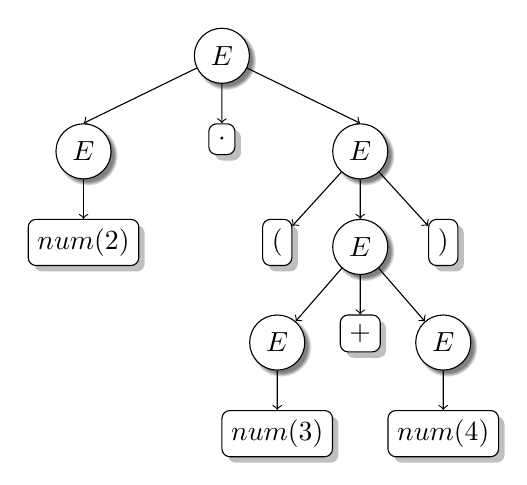
\begin{tikzpicture}[
    term/.style={rectangle, draw=black, rounded corners=1mm, fill=white, drop shadow,
        text centered, anchor=north, text=black},
    nonterm/.style={circle, draw=black, fill=white, circular drop shadow,
        text centered, anchor=north, text=black},
    level distance=0.5cm, growth parent anchor=south
]
\node (S0) [nonterm] {$E$} [->]
    [sibling distance=5em]
    child{ [sibling distance=2em]
    	node (S2) [nonterm] {$E$} [->]
	child{
		node (S4) [term] {$num(2)$}
	}
    }
    child {
    	node (S3) [term] {$\cdot$}
    }
    child{ [sibling distance=3em]
        node (S1) [nonterm] {$E$} [->]
        child{
		node (S6) [term] {$($}
	}
	child{
		node (S7) [nonterm] {$E$} [->]
		child{
			node (S9) [nonterm] {$E$} [->]
			child{
				node (S12) [term] {$num(3)$}
			}
		}
		child{
			node (S10) [term] {$+$}
		}
		child{
			node (S11) [nonterm] {$E$} [->]
			child{
				node (S13) [term] {$num(4)$}
			}
		}
	}
        child{
		node (S8) [term] {$)$}
	}
    }   
;
        
\end{tikzpicture}

\paragraph{Note} The quick introduction to CFGs presented here is certainly far from exhaustive. There are important issues of ambiguity and associativity of operations we have not considered at all so far. However, it should be sufficient to perform the required tasks. If you require more information or are simply interested feel free to look at \url{http://en.wikipedia.org/wiki/Context-free_grammar} and follow references from there.

\section{Tasks}

\subsection{Indexing}
\TODOP{Write description}

\subsection{Simple Search}
\TODOP{Write description}

\subsection{Sorting}
\TODOP{Write description}

\subsection{Queries}
Your query language should support \emph{union} and \emph{ordering}. It is described by the following CFG:
\begin{align*}
E &\to T &\mbox{ simple query}\\
E &\to T \ orderby \ Property \ Direction &\mbox{ ordering}\\
T &\to word &\mbox{ a search term} \\
T &\to T \ T &\mbox{ union} \\
Property &\to relevance &\mbox{ how often do the search terms appear in a document?}\\
Property &\to popularity &\mbox{ how popular is the document?}\\
Direction &\to asc &\mbox{ increasing order}\\
Direction &\to desc &\mbox{ decreasing order}
\end{align*}
\TODOP{Write the rest of the description}

\end{document}  